\documentclass[a4paper]{article}

\usepackage{caption}
\usepackage{amsmath}

\captionsetup[table]{position=bottom}

\setlength{\parindent}{0}

%\usepackage[cm]{fullpage}

% some very useful LaTeX packages include:

%\usepackage{cite}      % Written by Donald Arseneau
                        % V1.6 and later of IEEEtran pre-defines the format
                        % of the cite.sty package \cite{} output to follow
                        % that of IEEE. Loading the cite package will
                        % result in citation numbers being automatically
                        % sorted and properly "ranged". i.e.,
                        % [1], [9], [2], [7], [5], [6]
                        % (without using cite.sty)
                        % will become:
                        % [1], [2], [5]--[7], [9] (using cite.sty)
                        % cite.sty's \cite will automatically add leading
                        % space, if needed. Use cite.sty's noadjust option
                        % (cite.sty V3.8 and later) if you want to turn this
                        % off. cite.sty is already installed on most LaTeX
                        % systems. The latest version can be obtained at:
                        % http://www.ctan.org/tex-archive/macros/latex/contrib/supported/cite/
\usepackage[inline]{enumitem}

\usepackage{graphicx}   % Written by David Carlisle and Sebastian Rahtz
                        % Required if you want graphics, photos, etc.
                        % graphicx.sty is already installed on most LaTeX
                        % systems. The latest version and documentation can
                        % be obtained at:
                        % http://www.ctan.org/tex-archive/macros/latex/required/graphics/
                        % Another good source of documentation is "Using
                        % Imported Graphics in LaTeX2e" by Keith Reckdahl
                        % which can be found as esplatex.ps and epslatex.pdf
                        % at: http://www.ctan.org/tex-archive/info/

%\usepackage{psfrag}    % Written by Craig Barratt, Michael C. Grant,
                        % and David Carlisle
                        % This package allows you to substitute LaTeX
                        % commands for text in imported EPS graphic files.
                        % In this way, LaTeX symbols can be placed into
                        % graphics that have been generated by other
                        % applications. You must use latex->dvips->ps2pdf
                        % workflow (not direct pdf output from pdflatex) if
                        % you wish to use this capability because it works
                        % via some PostScript tricks. Alternatively, the
                        % graphics could be processed as separate files via
                        % psfrag and dvips, then converted to PDF for
                        % inclusion in the main file which uses pdflatex.
                        % Docs are in "The PSfrag System" by Michael C. Grant
                        % and David Carlisle. There is also some information
                        % about using psfrag in "Using Imported Graphics in
                        % LaTeX2e" by Keith Reckdahl which documents the
                        % graphicx package (see above). The psfrag package
                        % and documentation can be obtained at:
                        % http://www.ctan.org/tex-archive/macros/latex/contrib/supported/psfrag/

%\usepackage{subfigure} % Written by Steven Douglas Cochran
                        % This package makes it easy to put subfigures
                        % in your figures. i.e., "figure 1a and 1b"
                        % Docs are in "Using Imported Graphics in LaTeX2e"
                        % by Keith Reckdahl which also documents the graphicx
                        % package (see above). subfigure.sty is already
                        % installed on most LaTeX systems. The latest version
                        % and documentation can be obtained at:
                        % http://www.ctan.org/tex-archive/macros/latex/contrib/supported/subfigure/

\usepackage{url}        % Written by Donald Arseneau
                        % Provides better support for handling and breaking
                        % URLs. url.sty is already installed on most LaTeX
                        % systems. The latest version can be obtained at:
                        % http://www.ctan.org/tex-archive/macros/latex/contrib/other/misc/
                        % Read the url.sty source comments for usage information.

%\usepackage{stfloats}  % Written by Sigitas Tolusis
                        % Gives LaTeX2e the ability to do double column
                        % floats at the bottom of the page as well as the top.
                        % (e.g., "\begin{figure*}[!b]" is not normally
                        % possible in LaTeX2e). This is an invasive package
                        % which rewrites many portions of the LaTeX2e output
                        % routines. It may not work with other packages that
                        % modify the LaTeX2e output routine and/or with other
                        % versions of LaTeX. The latest version and
                        % documentation can be obtained at:
                        % http://www.ctan.org/tex-archive/macros/latex/contrib/supported/sttools/
                        % Documentation is contained in the stfloats.sty
                        % comments as well as in the presfull.pdf file.
                        % Do not use the stfloats baselinefloat ability as
                        % IEEE does not allow \baselineskip to stretch.
                        % Authors submitting work to the IEEE should note
                        % that IEEE rarely uses double column equations and
                        % that authors should try to avoid such use.
                        % Do not be tempted to use the cuted.sty or
                        % midfloat.sty package (by the same author) as IEEE
                        % does not format its papers in such ways.
\usepackage{amssymb}
\usepackage{amsmath}    % From the American Mathematical Society
                        % A popular package that provides many helpful commands
                        % for dealing with mathematics. Note that the AMSmath
                        % package sets \interdisplaylinepenalty to 10000 thus
                        % preventing page breaks from occurring within multiline
                        % equations. Use:
%\interdisplaylinepenalty=2500
                        % after loading amsmath to restore such page breaks
                        % as IEEEtran.cls normally does. amsmath.sty is already
                        % installed on most LaTeX systems. The latest version
                        % and documentation can be obtained at:
                        % http://www.ctan.org/tex-archive/macros/latex/required/amslatex/math/
\usepackage{latexsym}
\usepackage{amsthm}

\usepackage[utf8]{inputenc}
\usepackage[italian]{babel}

\usepackage{algorithm}
\usepackage{algpseudocode}
\algrenewcommand{\algorithmiccomment}[1]{$\left(\text{#1}\right)$}

\usepackage{color}

\definecolor{ideanumber}{rgb}{0.0,0.0,1.0}
\definecolor{ideacomment}{rgb}{0.5,0.5,0.5}
\definecolor{ideakeyword}{rgb}{0.0,0.0,0.5}
\definecolor{ideastring}{rgb}{0.0,0.5,0.0}

\usepackage{listings}
\lstset{frame=tb,
    language=Java,
    aboveskip=3mm,
    belowskip=3mm,
    showstringspaces=false,
    columns=flexible,
    basicstyle={\small\ttfamily},
    numbers=left,
    numbersep=2pt,                   % how far the line-numbers are from the code
    numberstyle=\tiny\color{ideacomment},
    keywordstyle=\color{ideakeyword},
    commentstyle=\color{ideacomment},
    stringstyle=\color{ideastring},
    breaklines=true,
    breakatwhitespace=true,
    tabsize=4
}

% Other popular packages for formatting tables and equations include:

%\usepackage{array}
% Frank Mittelbach's and David Carlisle's array.sty which improves the
% LaTeX2e array and tabular environments to provide better appearances and
% additional user controls. array.sty is already installed on most systems.
% The latest version and documentation can be obtained at:
% http://www.ctan.org/tex-archive/macros/latex/required/tools/

% V1.6 of IEEEtran contains the IEEEeqnarray family of commands that can
% be used to generate multiline equations as well as matrices, tables, etc.

% Also of notable interest:
% Scott Pakin's eqparbox package for creating (automatically sized) equal
% width boxes. Available:
% http://www.ctan.org/tex-archive/macros/latex/contrib/supported/eqparbox/

% *** Do not adjust lengths that control margins, column widths, etc. ***
% *** Do not use packages that alter fonts (such as pslatex).         ***
% There should be no need to do such things with IEEEtran.cls V1.6 and later.
\newcommand\textsup[1]{$^{\text{#1}}$}
\newcommand\textsub[1]{$_{\text{#1}}$}

% Define document title and author
\title{\LARGE \bf
Assigment \#2 - ``Asynchronous Programming''
}
\author{
    Martina Magnani\\
    \texttt{martina.magnani8@studio.unibo.it}
    \and
    Nicola Piscaglia\\
    \texttt{nicola.piscaglia2@studio.unibo.it}
    \and
    Mattia Vandi\\
    \texttt{mattia.vandi@studio.unibo.it}
}
\date{}

% Your document starts here!
\begin{document}

\maketitle
\section{Analisi del problema}\label{analisi-del-problema}

Progettare e implementare uno strumento per cercare corrispondenze di un'espressione regolare in una struttura ad albero o grafo di file (come un filesystem o un sito web).\\
Lo strumento deve avere il seguente comportamento:
\begin{itemize}
    \item Input\label{input}:
        \begin{itemize}
            \item Percorso di base della ricerca (ad esempio, un percorso del filesystem o un URL della pagina web)
            \item Espressione regolare
            \item Profondit� massima di ricerca
        \end{itemize}
    \item Output\label{output}:
        \begin{itemize}
            \item Elenco dei file corrispondenti
            \item Percentuale di file con almeno una corrispondenza (somma di file con corrispondenza/file totali);
            \item Numero medio di corrispondenze tra i file con corrispondenze (somma di tutte le corrispondenze/numero di file con corrispondenze).
        \end{itemize}
        Le uscite devono essere aggiornate in tempo reale con il procedere dell'elaborazione.
\end{itemize}
\\
\textbf{Esercizio 1}:\\
Risolvere il problema usando task ed executor
        \begin{itemize}
            \item I file devono essere letti e analizzati contemporaneamente.
            \item Si pu� anche optare per parallelizzare l'analisi di file di grandi dimensioni.
        \end{itemize}
\textbf{Esercizio 2}:\\
Risolvere il problema utilizzando la programmazione asincrona con Event Loop
        \begin{itemize}
            \item Cerca di riutilizzare il maggior numero possibile di codice dall'esercizio 1, ma anche di ripensare alla soluzione in base al nuovo punto di vista.
        \end{itemize}
\textbf{Esercizio 3}:\\
Risolvere il problema utilizzando i flussi reattivi
        \begin{itemize}
            \item Ad esempio, i risultati dell'elaborazione possono essere reificati in un flusso di eventi che pu� essere manipolato mediante tecniche di programmazione reattiva
        \end{itemize}
\\
\textbf{Ulteriori note}:
\begin{itemize}
    \item L'interfaccia utente pu� essere a riga di comando, grafica o basata sul web. 
    \item Sei libero di utilizzare qualsiasi framework basato sugli eventi (ad es. Vertx, NodeJS) e la libreria del flusso reattivo (ad es. RxJava, Sodio).
\end{itemize}

\section{Descrizione della soluzione proposta}\label{descrizione-della-soluzione-proposta}
Lo strumento realizzato serve per la ricerca di corrispondenze di un'espressione regolare tra i file, dato un percordo di partenza e la profondit� massima. 
\subsection{Design}\label{design}
\subsubsection{Dominio Applicativo}
L'architettura del sistema � stata realizzata in modo che il dominio applicativo fosse svincolato dalla logica di controllo e fosse condiviso fra le tre soluzioni.\\\\
Il dominio applicativo � composto dai seguenti elementi:
\begin{itemize}
    \item \texttt{Document}: classe che astrae il concetto di documento, � composto da una lista ordinata di linee che rappresentano il suo contenuto e dal nome del documento.
    \item \texttt{Folder} classe che astrae il concetto di cartella di un filesystem, � composta da una lista di documenti e da una lista di sottocartelle.
    \item \texttt{SearchResult}: classe che rappresenta il risultato della ricerca delle occorrenze dell'espressione regolare (fornita in input) in uno specifico documento. Il risultato � composto dal nome del documento e dal numero di occorrenze trovate.
    \item \texttt{SearchStatistics}: classe che rappresenta le statistiche della ricerca in atto come richieste nell'Output specificato nell'analisi del problema \ref{output}. 
\end{itemize}
\subsubsection{Esercizio 1: Task & Executors}
La soluzione proposta vede l'utilizzo del modello ForkJoin, questo ci permette di suddividere il problema in una gerarchia di compiti atomici.
Analizzando i requisiti abbiamo individuato tre task principali:
\begin{itemize}
    \item \texttt{FolderSearchTask}: ricerca delle occorrenze dell'espressione regolare in una cartella
    \item \texttt{DocumentSearchTask}: ricerca delle occorrenze dell'espressione regolare in un documento
    \item \texttt{SearchResultAccumulatorTask}: aggregazione dei risultati e calcolo delle statistiche
\end{itemize}
Dato un percorso e una profondit� massima viene costruito un albero nel quale le cartelle rappresentano i rami e i documenti le foglie. Partendo dalla radice visitiamo tutte le sottocartelle e i documenti presenti: nel primo caso viene eseguito un nuovo \texttt{FolderSearchTask}, nel secondo caso viene eseguito un nuovo \texttt{DocumentSearchTask}.\\
Ogni risultato intermedio trovato mette in esecuzione una callback che notifica il \texttt{SearchResultAccumulatorTask}, eseguito su un executor dedicato.\\
\texttt{SearchResultAccumulatorTask} si occupa di aggiornare i risultati e di passarli ad una callback responsabile di aggiornare l'output.  

\subsubsection{Esercizio 2: Event Loop}

\subsubsection{Esercizio 3: Reactive Streams}
Come implementazione dei flussi reattivi abbiamo usato la libreria RxJava2 \footnote{\url{https://github.com/ReactiveX/RxJava}}.
L'approccio dichiarativo fornito dall'utilizzo dei Reactive Stream permette di semplificare la soluzione.
In questo caso l'insieme di documenti � visto come flusso reattivo al quale � possibile applicare operazioni di trasformazione, di calcolo e di sottoscrizione.  
Abbiamo scelto di utilizzare i Flowable perch� implementano i reactive stream e il meccanismo di backpressure che permette di ottimizzare l'elaborazione del flusso di dati.\\
Lo stream di dati � stato creato a partire dalla radice dell'albero di cartelle: con il metodo \texttt{getDocuments()} otteniamo ricorsivamente i documenti di ogni cartella e sottocartella e li mappiamo in un unico stream di documenti.

Generato lo stream specifichiamo su quale Scheduler verrano eseguite le manipolazioni.

Per ogni documento dello stream contiamo il numero di occorrenze dell'espressione regolare in input e lo trasformiamo in un \texttt{SearchResult}.

A questo punto sottoscriviamo \texttt{SearchResultAccumulator} al flusso utilizzando \texttt{blockingSubscribe()}: questa scelta � dovuta al fatto che vogliamo sospenderci sul thread corrente finch� tutto lo stream non � stato processato.

\texttt{SearchResultAccumulator} implementa l'interfaccia \texttt{Subscriber}, che gli permette di essere notificato quando un nuovo elemento del flusso � disponibile e della sua terminazione.
All'arrivo di un nuovo dato si occupa di aggiornare i risultati e della creazione delle statistiche. Quest'ultime vengono passate ad una callback responsabile dell'aggiornamento dell'output.

\section{Dinamica del sistema}\label{dinamica-del-sistema}
La dinamica del sistema � stata rappresentata formalmente con le Reti di Petri. Le piazze (\textit{places}) del livello corrispondono ai \texttt{Worker} che concorrono all'aggiornamento della scacchiera di gioco; in questo esempio � stato scelto di mostrare il sistema nel caso se ne utilizzino 4.
\begin{figure}[H]
    \centering
    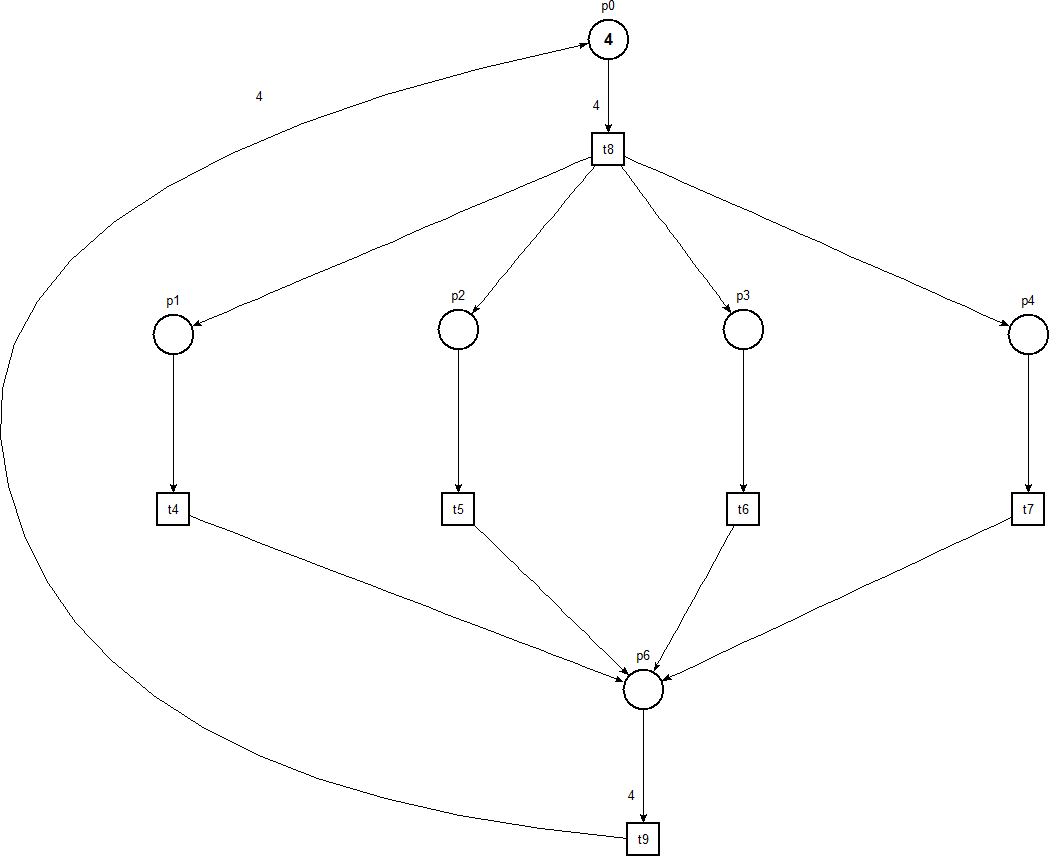
\includegraphics[width=110mm]{res/reti_di_petri_assigment1.png}
    \caption{Petri Net}
    \label{fig:petrinets}
\end{figure}

\section{Analisi delle prestazioni}\label{analisi-delle-prestazioni}

\begin{table}[H]
\centering
\begin{tabular}{l|ccccccccc}
\hline
     & 2     & 3    & 4    & 5    & 6    & 7    & 8    & 9    & 10   \\ \hline
Min. & 1.77  & 2.43 & 3.04 & 2.93 & 2.89 & 2.90 & 2.86 & 2.85 & 2.85 \\
Max. & 2.11  & 2.87 & 3.41 & 3.22 & 3.40 & 3.26 & 3.38 & 3.06 & 3.45 \\
Avg. & 1.81  & 2.50 & 3.06 & 2.94 & 2.93 & 2.91 & 2.92 & 2.85 & 2.94 \\ \hline
\end{tabular}
\caption{Speedup considerando schacchiera di gioco 5000x5000: sulle colonne sono specificati il numero di worker utilizzati per la parallelizzazione dell'algoritmo, sulle righe i valori statistici (minimi, massimi e medi) degli speedup calcolati. Gli speed-up sono stati calcolati su un Apple Macbook Pro (Retina, 15", met� 2015) dotato di un processore Intel Core i7 quad-core a 2.2GHz.}
\label{Tabella speedup del sistema}
\end{table}

% Your document ends here!
\end{document}
